\section{Návrh}

% prva uroven abstrakcie
Chceme pomocou neurónovej siete namodelovať funkciu ktorá nám povie, po istom počte písmen aké je najpravdepodobnejšie ďalšie písmeno. Takýmto spôsobom budeme vedieť generovať texty. Celý proces môžeme rozdeliť na dve podúlohy, prvá je trénovanie modelu, kedy sa model učí a druhá podúloha je generovanie, pri ktorom model na základe naučeného predpovedá.

Na trénovanie budeme potrebovať dáta, z ktorých sa náš model vie naučiť pravdepodobnostné rozloženie písmen. Pre tento prípad sme si zvolili Wikipédiu, kvôli svojej rozmanitosti a veľkosti. Model na vstup dostane sekvenciu znakov a bude musieť predpovedať sekvenciu znakov posunutú o jeden znak ďalej, takto sa naučí ako z aktuálnej sekvencie vygenerovať ďalšiu sekvenciu s pridaným znakom.

Na generovanie si môžeme vstupnú sekvenciu vymyslieť, môže to byť písmeno alebo celé slovo. A už trénovaná sieť bude vedieť povedať, pravdepodobnosti toho aké by malo byť ďalšie písmeno v poradí. Príkladom môže byť že mu na vstup zadáme sekvenciu "abc" a sieť vráti pravdepodobnosti pre celý slovník v tomto prípade iba a,b,c s prislúchajúcimi hodnotami ich pravdepodobnosti výskytu ako ďalšie písmeno(napr. 0.2, 0.2, 0.6) potom je už na nás, ktoré si vyberieme a ako.

% Budeme trénovať neurónovú sieť a našim cieľom bude namodelovať pravdepodobnostné rozloženie jednotlivých písmen v slovenčine a angličtine a následne pomocou tohto štatistického rozdelenia generovať n-gramy t.j. text znak po znaku pričom budeme brať do úvahy nie len predchádzajúce prímeno ale všetky predchádzajúce písmená. Návrh sa teda skladá z dvoch častí z trénovania a následného generovanie. Pri trénovaní získame pravdepodobnostné rozdelenie písmen a pri generovaní pomocou tohto rozdelenia budeme predpovedáme nasledujúce písmeno v poradí.

% druha uroven abstrakcie
% dataset
% model obr

\subsection{Dataset}
% Z IITSRC

\subsection{Opis Modelu}
Tým pádom že modelujeme sekvenciu znakov a závisí nám aj od predchádzajúcich  vstupoch nie len na konkrétnom použijeme rekurentnú neurónovú sieť. Konkrétne LSTM siete, ktoré nemajú problém s dlhodobými závislosťami vstupov.

Na modelovanie a generovanie použijeme model znázornení na obrázku \ref{fig:nn_model}. Vstup do siete bude kódovaní ako one-hot vektor (každé písmeno má priradení index) tento vstup sa posunie do Embedding vrstvy, ktorá má za úlohu naučiť sa vektorové reprezentácie pomocou desatinnými číslami pre jednotlivé vstupy, táto reprezentácia sa potom posunie do LSTM vrstvy. Nakoniec výstup posunieme do lineárnej vrstvy ktorá nám zredukuje výstup z LSTM vrstiev na vhodnú veľkosť, ktorý potom môžeme interpretovať ako vektor pravdepodobnostných hodnoty pre jednotlivé možné vstupy.

Konfigurácia siete je nasledujúca:
embedding vrstva nám vráti vektor s 200 dimenziami
máme 2 vrstvy LSTM sietí, s veľkosťou 200 neuŕonov
a na konci použijeme softmax

\subsection{Trénovanie Modelu}

Náš model budeme trénovať na slovenskom a anglickom texte, korpus použijeme z wikipédie. Kvôli rozdielom vo veľkosti slovenskej a anglickej wikipédie použijeme voľne dostupné texty slovenskej a simplifikovanej anglickej wikipédie.

Trénovanie siete potom prebieha tak že každému písmenu pridelíme index(one-hot vektor) zo slovníka a následne ich pošleme do nášho modelu. Výslednú hodnotu porovnáme s ďalšou v poradí, váhy sa vhodne upravia

Celú sieť trénujeme na slovenskej a anglickej wikipédie. Kvôli rozdielom vo veľkosti a kvality slovenskej a anglickej wikipádii použijeme len simple english wikipédiu, ktorá má porovnateľnú veľkosť.

\subsection{Generovanie Textu}
V tejto fáze natrénovanej sieti pošleme písmeno a z výstupu siete zistíme písmeno s najvyššou hodnotou pravdepodobnosti, ktoré sa by sa mohlo vyskytnúť po vstupe tento výstup použijeme ako ďalší vstup do siete, takto pokračujeme, kým nemáme dostatočné množstvo textu viď obr. \ref{fig:nn_gen}.
% \begin{table}[]
% \begin{tabular}{|l|}
% \hline
% \begin{tabular}[c]{p{\linewidth}}John Cheerny\\John Leyn Show (August 24, 1940 0 February 23, 1987) was an American singer-songwriter and worldwide. He acted in the band for songs for the 1990s to the "Michael Albert Andrew \& Ort". He was set during the mid-1990s. He won a former club which became a character for the business Adele Shelley dollar women's song book "Raw" as NXT War Railway from the 2001 census.
% \end{tabular} \\ \hline
% \begin{tabular}[c]{p{\linewidth}}Saint-Martin\\ Saint-Maritre je francúzska obec, ktorá sa nachádza v departemente Orne, v regióne Dolná Normandia.\\ Obec má rozlohu . Najvyšší bod je položený a najnižší bod\\ Počet obyvateľov obce je ().\\ Nasledujúci graf zobrazuje vývoj počtu obyvateľov v obci.\end{tabular}                                                                                                                        \\ \hline
% \end{tabular}
% \caption{\label{tab:gen-text}Ukážka vygenerovaného slovenského a anglického textu.}
% \end{table}

\usetikzlibrary{positioning}

% \begin{figure}[ht]
% \centering



% \begin{tikzpicture}
% 	\node[rectangle] (Y0) at (0, 0) {$\dots$};
	
% 	\node[rectangle, draw, right=2em of Y0, minimum height=1cm, minimum width=1cm] (RNN) {NN};
% 	\node[rectangle, right=of RNN, draw, minimum height=1cm, minimum width=1cm] (RNN2) {NN};
% 	\node[rectangle, right=of RNN2, draw, minimum height=1cm, minimum width=1cm] (RNN3) {NN};
% 	\node[rectangle, right=2em of RNN3] (RNN4) {$\dots$};
			
% 	\node[below=of RNN] (X1) {'c'};
% 	\node[below=of RNN2] (X2) {'a'};
% 	\node[below=of RNN3] (X3) {'t'};
	
% 	\node[above=of RNN] (Y2) {'a'};
% 	\node[above=of RNN2] (Y3) {'t'};
% 	\node[above=of RNN3] (Y4) {'.'};
			
% 	\draw[-stealth, thick] (X1) -- (RNN);
% 	\draw[-stealth, thick] (RNN) -- (Y2);
	
% 	\draw[-stealth, thick]
% (RNN) edge[out=90,in=270, looseness=2] node[pos=0.55,yshift=5pt] {} (RNN2);

%     \draw[-stealth, thick] (X2) -- (RNN2);
% 	\draw[-stealth, thick] (RNN2) -- (Y3);

% 	\draw[-stealth, thick]
% (RNN2) edge[out=90,in=270, looseness=2] node[pos=0.55,yshift=5pt] {} (RNN3);

%     \draw[-stealth, thick] (X3) -- (RNN3);
% 	\draw[-stealth, thick] (RNN3) -- (Y4);

% 	\node[below=4em of Y0] (d) {\dots};
% 	\node[below=4em of RNN4] (d) {\dots};
% \end{tikzpicture}
%     \caption{Spôsob generovanie písmen na základe predchádzajúcich písmen}
%     \label{fig:nn_gen}
% \end{figure}

\begin{figure}[H]
\begin{center}
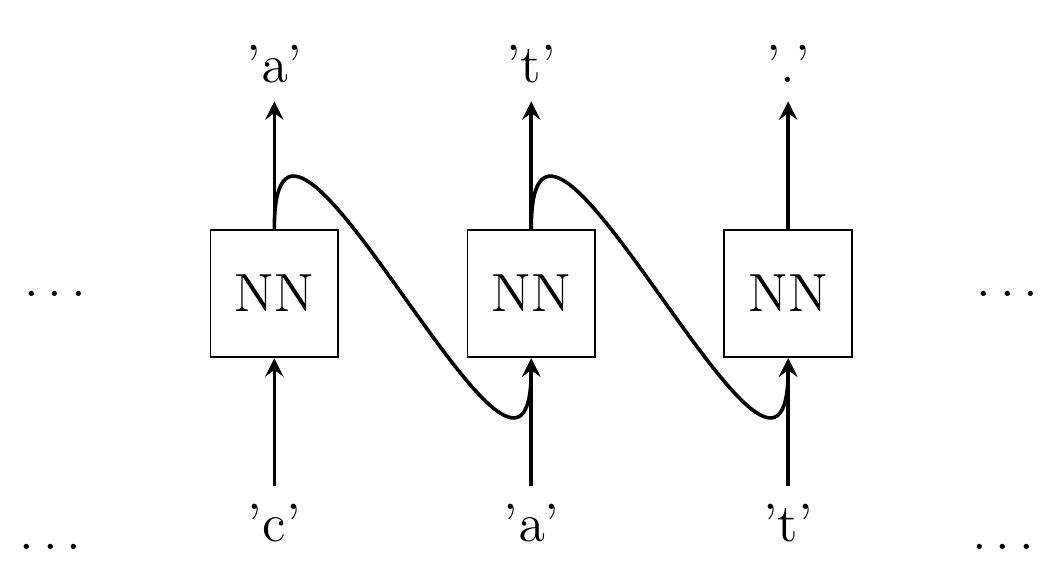
\includegraphics[width=1.0\linewidth]{figures/model-2.png}
\caption{Spôsob generovanie písmen na základe predchádzajúcich písmen}
\label{fig:nn_gen}
\end{center}
\end{figure}

% \begin{figure}[ht]
% \centering


% \begin{tikzpicture}
% 	\node[rectangle] (Y0) at (0, 0) {$\dots$};
	
% 	\node[rectangle, draw, right=2em of Y0, minimum height=1cm, minimum width=1cm] (RNN) {LSTM};
% 	\node[rectangle, right=of RNN, draw, minimum height=1cm, minimum width=1cm] (RNN2) {LSTM};
% 	\node[rectangle, right=of RNN2, draw, minimum height=1cm, minimum width=1cm] (RNN3) {LSTM};
% 	\node[rectangle, right=2em of RNN3] (RNN4) {$\dots$};
			
% 	\node[rectangle, above=of RNN, draw, minimum height=1cm, minimum width=1cm] (R22) {LSTM};
% 	\node[rectangle, right=of R22, minimum height=1cm, minimum width=1cm, draw] (R23) {LSTM};
% 	\node[rectangle, right=of R23, draw, minimum height=1cm, minimum width=1cm] (R24) {LSTM};
	
% 	\node[rectangle, above=of R22, draw, minimum height=1cm, minimum width=1cm] (LIN1) {Linear};
% 	\node[rectangle, above=of R23, draw, minimum height=1cm, minimum width=1cm] (LIN2) {Linear};
% 	\node[rectangle, above=of R24, draw, minimum height=1cm, minimum width=1cm] (LIN3) {Linear};
	
% 	\node[rectangle, below=of RNN, draw, minimum height=1cm, minimum width=1cm] (EMB1) {Embed};
% 	\node[rectangle, below=of RNN2, draw, minimum height=1cm, minimum width=1cm] (EMB2) {Embed};
% 	\node[rectangle, below=of RNN3, draw, minimum height=1cm, minimum width=1cm] (EMB3) {Embed};

% 	\node[rectangle, left=2em of R22] (R21) {$\dots$};
% 	\node[right=2em of R24] (Y20) {$\dots$};
			
% 	\node[below=of EMB1] (X1) {$\vec{x}_{t-1}$};
% 	\node[below=of EMB2] (X2) {$\vec{x}_t$};
% 	\node[below=of EMB3] (X3) {$\vec{x}_{t+1}$};
% 	\node[above=of LIN3] (Y4) {$\vec{y}_{t+1}$};
% 	\node[above=of LIN2] (Y3) {$\vec{y}_t$};
% 	\node[above=of LIN1] (Y2) {$\vec{y}_{t-1}$};
			
% 	\draw[-stealth, thick] (X1) -- (EMB1);
% 	\draw[-stealth, thick] (X2) -- (EMB2);
% 	\draw[-stealth, thick] (X3) -- (EMB3);
% 	\draw[-stealth, thick, densely dotted] (Y0) -- (RNN);
	
% 	\draw[stealth-, thick] (RNN2) -- node[above, pos=0.55] {$\vec{h^1}_{t-1}$} (RNN);
% 	\draw[stealth-, thick] (RNN3) -- node[above, pos=0.55] {$\vec{h^1}_t$} (RNN2);
	
% 	\draw[-stealth, densely dotted, thick] (RNN3) -- (RNN4);
% 	\node[below=4em of Y0] (d) {\dots};
% 	\node[below=4em of RNN4] (d) {\dots};

% 	\draw[-stealth, thick] (LIN1) -- (Y2);
% 	\draw[-stealth, thick] (LIN2) -- (Y3);
% 	\draw[-stealth, thick] (LIN3) -- (Y4);
	
% 	\draw[-stealth, thick] (R22) -- (LIN1);
% 	\draw[-stealth, thick] (R23) -- (LIN2);
% 	\draw[-stealth, thick] (R24) -- (LIN3);
	
% 	\draw[-stealth, thick] (EMB1) -- (RNN);
% 	\draw[-stealth, thick] (EMB2) -- (RNN2);
% 	\draw[-stealth, thick] (EMB3) -- (RNN3);
		
% 	\draw[stealth-, densely dotted, thick] (R22) -- (R21);
% 	\draw[stealth-, thick] (R23) -- node[above, pos=0.55] {$\vec{h^2}_{t-1}$} (R22);
% 	\draw[stealth-, thick] (R24) -- node[above, pos=0.55] {$\vec{h^2}_t$} (R23);
% 	\draw[-stealth, densely dotted, thick] (R24) -- (Y20);	
			
% 	\draw[stealth-, thick] (R22) -- node[left, pos=0.55] {$\vec{o^1}_{t-1}$}(RNN);
% 	\draw[stealth-, thick] (R23) -- node[left, pos=0.55] {$\vec{o^1}_t$}(RNN2);
% 	\draw[stealth-, thick] (R24) -- node[left, pos=0.55] {$\vec{o^1}_{t+1}$}(RNN3);
	
% 	\draw[stealth-, thick] (LIN1) -- node[left, pos=0.55] {$\vec{o^2}_{t-1}$}(R22);
% 	\draw[stealth-, thick] (LIN2) -- node[left, pos=0.55] {$\vec{o^2}_t$}(R23);
% 	\draw[stealth-, thick] (LIN3) -- node[left, pos=0.55] {$\vec{o^2}_{t+1}$}(R24);
% \end{tikzpicture}

%     \caption{Model neurónovej siete na generovanie textu}
%     \label{fig:nn_model}
% \end{figure}

\begin{figure}[H]
\begin{center}
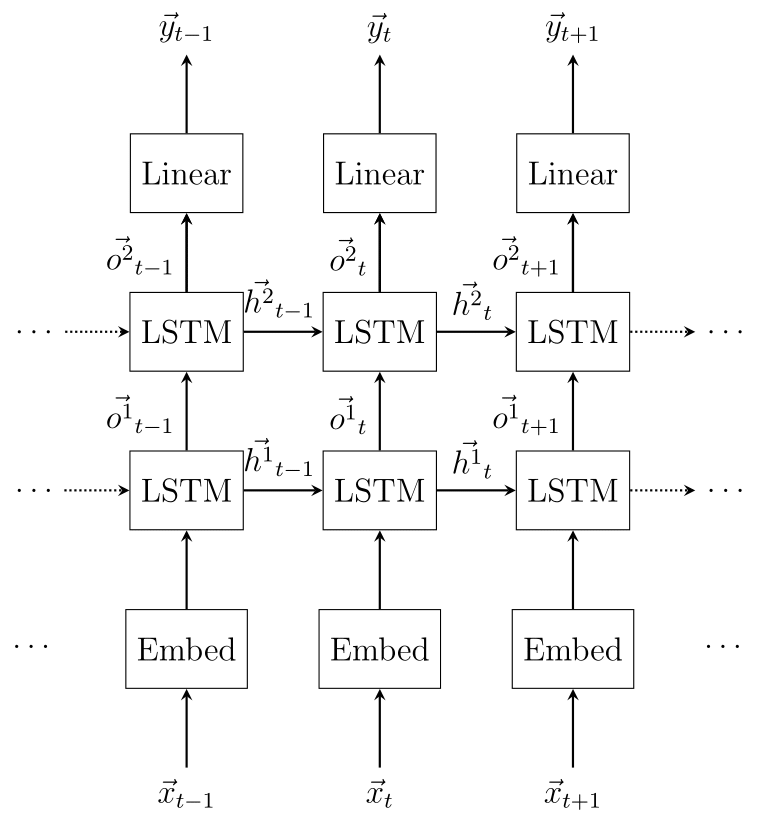
\includegraphics[width=1.0\linewidth]{figures/model-1.png}
\caption{Model neurónovej siete na generovanie textu}
\label{fig:nn_model}
\end{center}
\end{figure}

% tretia uroven abstrakcie - kod

\subsection{implementácia}
Na implementáciu použijeme programovací jazyk Python a na uľahčenie práce s neurónovými sieťami knižnicu PyTorch, ktorá obsahuje väčšinu potrebných komponentov na poskladanie modelu.

\subsubsection{predspracovanie}
% IITSRC

\subsubsection{model}
% model.py

\subsubsection{trénovanie}
% train.py

\subsubsection{generovanie}
% generate.py